\documentclass[10pt,twocolumn]{article}

\usepackage{fullpage}
\usepackage{times}
\usepackage{multirow}
\usepackage{arydshln}
\usepackage{amssymb,amsmath}
\usepackage{ifxetex,ifluatex}
\usepackage{amsmath}
\usepackage{mathptmx}
\usepackage{graphicx}
\usepackage{listings}



% use upquote if available, for straight quotes in verbatim environments
\IfFileExists{upquote.sty}{\usepackage{upquote}}{}

\usepackage{graphicx}
\usepackage[font=footnotesize,labelfont=bf]{caption}
\usepackage{pstricks}
\makeatletter
\def\maxwidth{\ifdim\Gin@nat@width>\linewidth\linewidth\else\Gin@nat@width\fi}
\def\maxheight{\ifdim\Gin@nat@height>\textheight\textheight\else\Gin@nat@height\fi}
\makeatother
% Scale images if necessary, so that they will not overflow the page
% margins by default, and it is still possible to overwrite the defaults
% using explicit options in \includegraphics[width, height, ...]{}
\setkeys{Gin}{width=\maxwidth,keepaspectratio}
\ifxetex
  \usepackage[setpagesize=false, % page size defined by xetex
              unicode=false, % unicode breaks when used with xetex
              xetex]{hyperref}
\else
  \usepackage[unicode=true]{hyperref}
\fi
\hypersetup{breaklinks=true,
            bookmarks=true,
            pdfauthor={},
            pdftitle={Malacology: A Programmable Storage System Built on Ceph},
            colorlinks=true,
            citecolor=blue,
            urlcolor=blue,
            linkcolor=black,
            pdfborder={0 0 0}}
\urlstyle{same}  % don't use monospace font for urls
%\setlength{\parindent}{0pt}
%\setlength{\parskip}{6pt plus 2pt minus 1pt}
%\setlength{\emergencystretch}{3em}  % prevent overfull lines
\setcounter{secnumdepth}{5}

\title{Malacology: A Programmable Storage System Built on Ceph}
\author{Paper \# 123}
\date{}
\begin{document}

\maketitle

\begin{abstract}
Storage systems are caught between rapidly changing data processing systems and
the increasing speed of storage devices. This puts tremendous pressure on
storage systems to adapt both in terms of their interfaces and their
performance. But adapting storage systems can be difficult because unprincipled
changes might jeopardize years of code-hardening and performance optimization
efforts that were necessary for users to entrust their data to the storage
system.  We introduce  Malacology, a prototype programmable storage system to
explore how existing abstractions of common services found in storage systems
can be leveraged to address new data processing systems and the increasing
speed of storage devices. This approach allows unprecedented flexibility for
storage systems to evolve without sacrificing the robustness of its
code-hardened subsystems.  We illustrate the advantages and challenges of
programmability by constructing two services out of existing abstractions: a
file system metadata load balancer and a high-performance distributed shared-log
that leverages flash devices. The evaluation demonstrates that our services 
inherit desirable qualities of Ceph, including the ability to make trade-offs 
for lease capabilities, balance load (2\(\times\) improvement), propagate interfaces 
(average of 222ms) and recover (15 second down time).  
\end{abstract}

\section{Introduction}
\label{introduction}
\label{sec:intro}

A storage system implements abstractions designed to persistently store
data and must exhibit a high level of correctness to prevent data loss.
Storage systems have evolved around storage devices that often were
orders of magnitude slower than CPU and memory, and therefore could
dominate overall performance if not used carefully. Over the last few
decades members of the storage systems community have developed
ingenious strategies to meet correctness requirements while somewhat
hiding the latency of traditional storage media~\cite{brewer_disks_2016}. To avoid lock-in by a
particular vendor, users of storage systems have preferred systems with
highly standardized APIs and lowest common denominator abstract data
types such as blocks of bytes and byte stream files~\cite{armbrust_view_2010}.

A number of recent developments are disrupting traditional storage
systems: (1) the falling prices of flash storage and the availability of
new types of non-volatile memory that are orders of magnitude faster
than traditional spinning media are moving overall performance
bottlenecks away from storage devices to CPUs and networking, and
pressure storage systems to shorten their code paths and incorporate new
optimizations~\cite{gray_tape_2007,gray_flash_2008}; (2) demand for managing structured data and flexible
consistency semantics at scale pressure big data processing systems to
use storage abstractions that can meet these demands~\cite{apache_contributors_parquet_2014}; and (3)
production-quality scalable storage systems available as open source
software have established and are continuing to establish new, \emph{de-facto} API standards at a faster pace than traditional standards bodies~\cite{snia_implementing_2014,linux_foundation_kinetic_2015}.

\begin{figure}[tb]
\centering
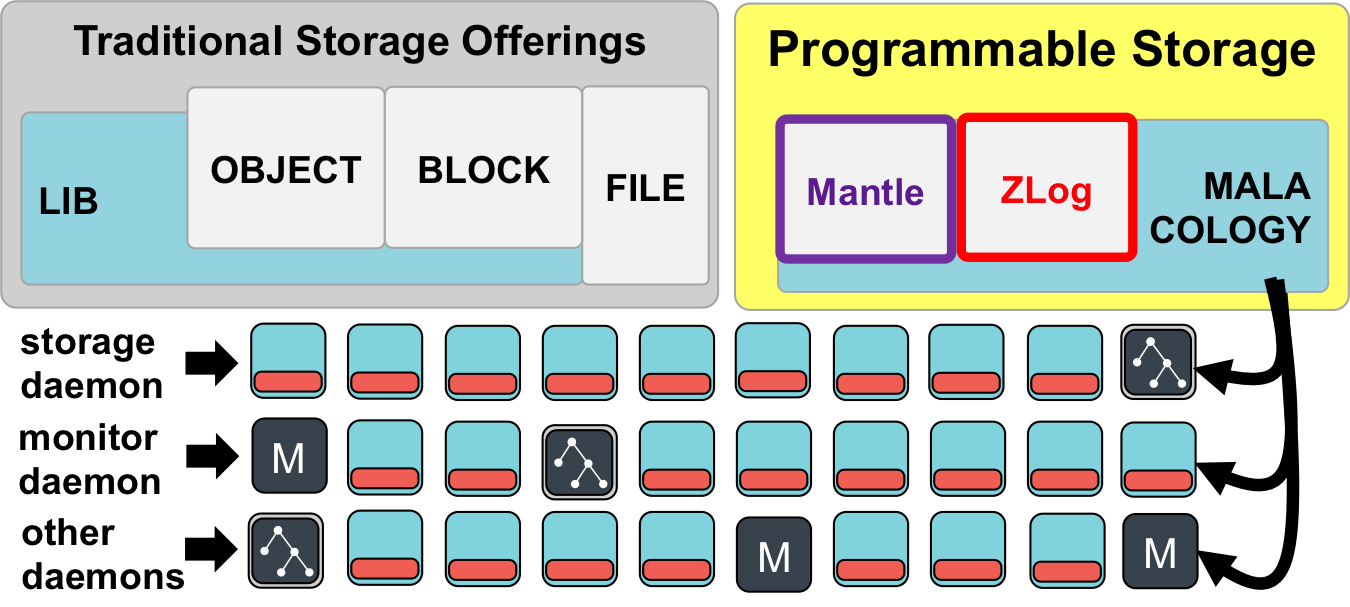
\includegraphics{figures/overview.png}
\caption{A Ceph installation consists of a cluster running mostly
storage daemons (OSDs) to ensure data durability, a few monitor daemons
(MONs) to reach consensus of the cluster state and to ensure its
consistent versioning, and a few metadata service daemons (MDSs) for
scalable metadata service. Ceph's APIs include object, block, file
abstractions. Malacology enables the programmability of these
abstractions and services (indicated by bold arrows). To illustrate Malacology we implement two
services on Ceph, ZLog and Mantle, by programming Ceph's durability,
consistent versioning, consensus, and metadata subsystems.
\label{fig:overview}}
\end{figure}

These three trends put evolutionary pressure on storage systems and
raise the question whether there are principles that storage systems
designers can follow to evolve storage systems efficiently and without
jeopardizing years of code-hardening and performance optimization
efforts that are important for users to continue to entrust their data
to the storage system.

In this paper we investigate an approach that focuses on generalizing
existing storage system resources, services, and abstractions that in
generalized form can be used to \emph{program} new services. By doing so
one can reuse subsystems and leverage their optimizations,
established correctness, robustness, and efficiency. We will refer to
this programmability as \emph{programmable storage}, which differs from
\emph{active storage} (the injection and execution of arbitrary code in
a storage system) and \emph{software-defined storage} (the control of
thin-provisioning of storage).

To illustrate the benefits and challenges of this approach we examine
the programmability of Ceph~\cite{weil:osdi2006-ceph,ceph}, the increasingly
popular, production-level open-source distributed storage system.
Something of a storage swiss army knife, Ceph supports file, block, and
object interfaces simultaneously in a single cluster~\cite{ceph_contributors_ceph_2010}. Ceph's Reliable Autonomous 
Distributed Object Storage (RADOS) system is a cluster of storage
devices (OSDs) that provide Ceph with data durability and integrity
using replication, erasure-coding, and scrubbing~\cite{weil_rados_2007}. 
% By introducing
% programmability concepts into Ceph, we can build new services by
% carefully exposing internal storage services to applications.

Ceph also provides empirical evidence that developers embrace programmable storage: Ceph already supports the
implementation of domain-specific logical object interfaces by composing
existing interfaces. These interfaces are written in C++ and are statically
loaded into the system. Figure~\ref{fig:obj-int-dev-growth} shows a dramatic growth in the production use of
domain-specific interfaces in the Ceph community since 2010.  What is most
remarkable is that this trend contradicts the notion that API changes are a
burden for users.
Rather it appears that a gap in existing interfaces are
being addressed through programmability. In fact, Table~\ref{table:objclasses}
categorizes existing interfaces and we clearly see a trend towards reusable
services.

\begin{figure}[ht]
\centering
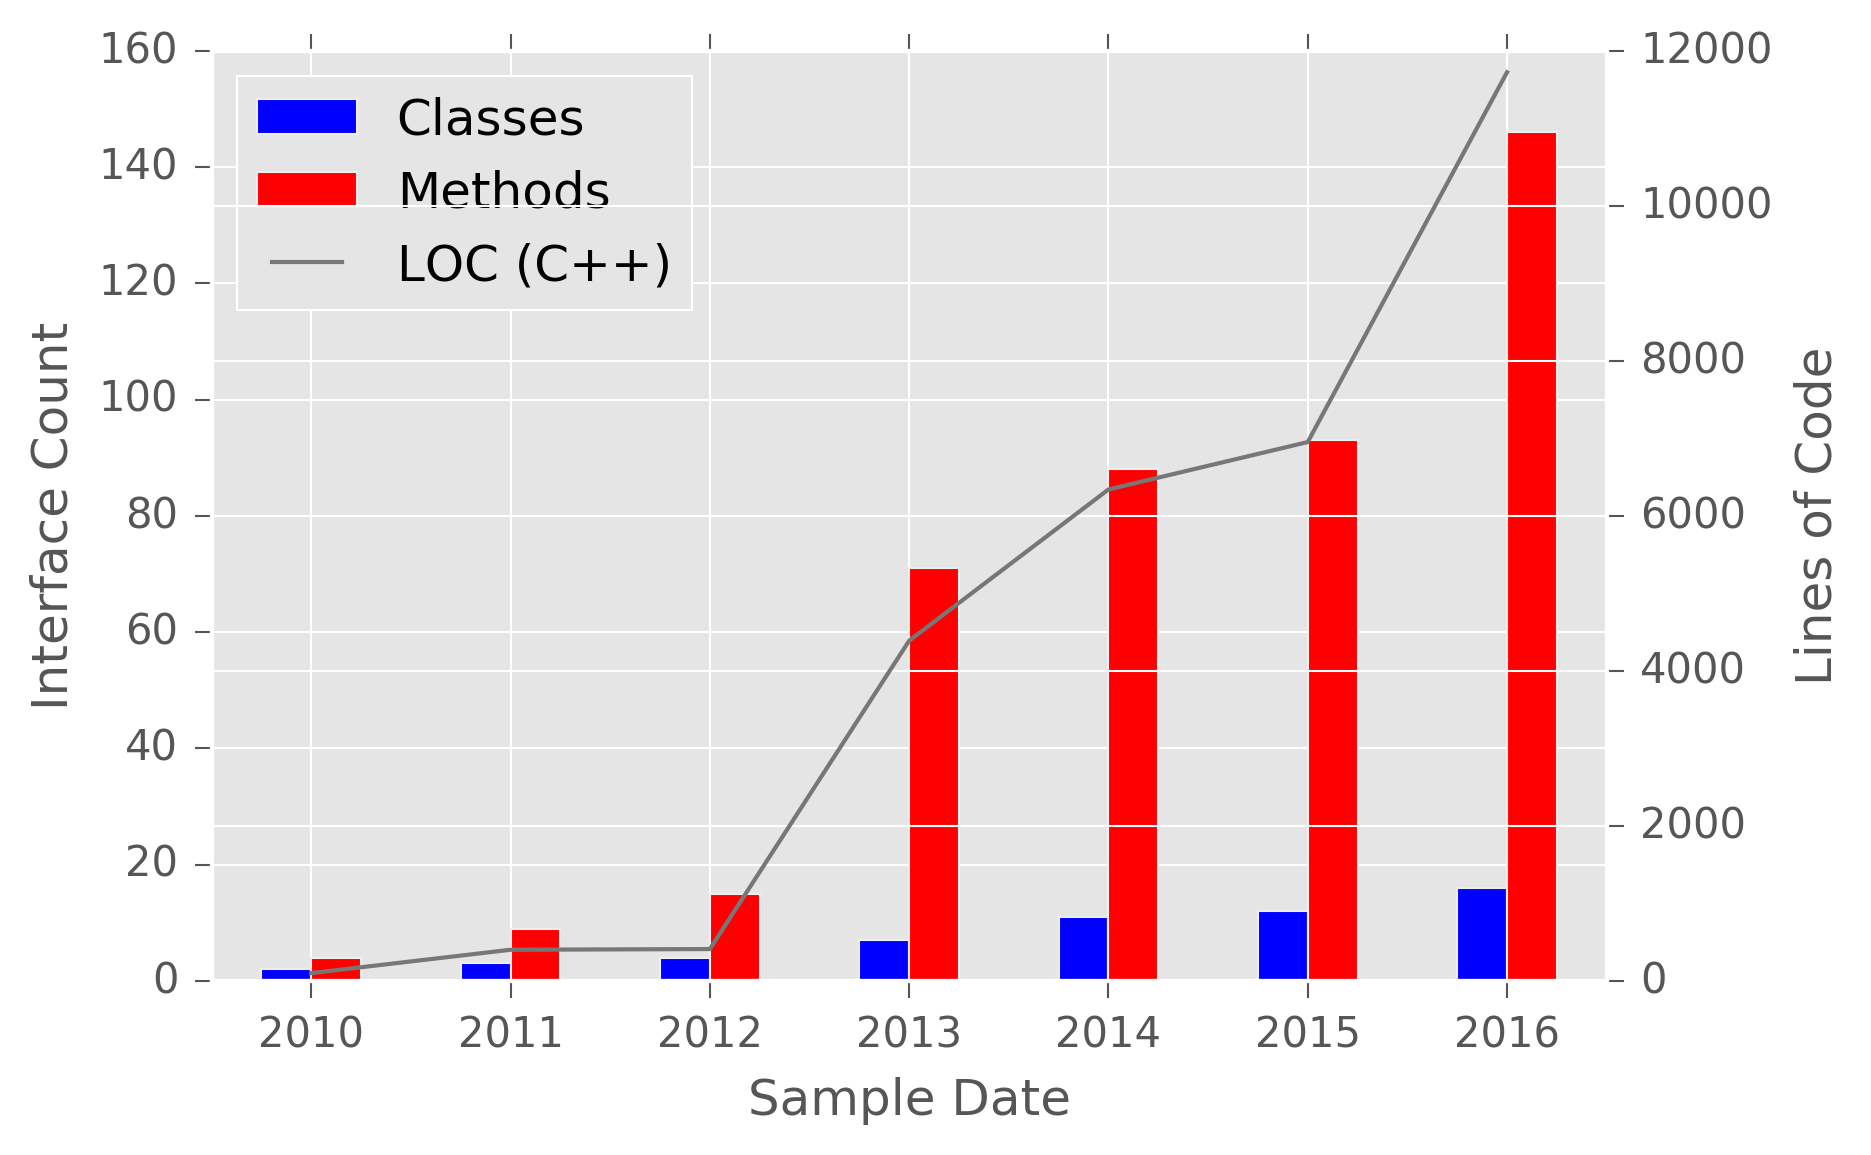
\includegraphics{figures/obj-int-dev-growth.png}
\caption{Since 2010, the growth in the number of co-designed object
storage interfaces in Ceph has been accelerating. This plot is the
number of object classes (a group of interfaces), and the total number
of methods (the actual API end-points).}
\label{fig:obj-int-dev-growth}
\end{figure}

\begin{table}[ht]
\centering
  \begin{tabular}{l|l|l}
    Category & Specialization& \# \\ \hline
    \multirow{2}{*}{Locking} & Shared & \multirow{2}{*}{6} \\
                             & Exclusive & \\ \hdashline
    \multirow{3}{*}{Logging} & Replica & 3 \\
                             & State & 4 \\
                             & Timestamped & 4 \\ \hdashline
    \multirow{4}{*}{Metadata Managment} 
                             & RADOS Block Device  & 37 \\
                             & RADOS Gatway & 27 \\
                             & User & 5 \\
                             & Version & 5 \\ \hdashline
    Garbage Collection       & Reference Counting & 4 \\
\end{tabular}
\caption{A variety of RADOS object storage classes exist to expose interfaces
    to applications. \# is the number of methods that use these categories.
}
\label{table:objclasses}
\end{table}

The popularity of the custom object interface facility of Ceph hint at three
trends in the Ceph community: (1) increasingly, the default
algorithms/tunables of the storage system are insufficient for the
application's performance goals, (2) programmers are becoming more aware
of their application's behavior, and (3) programmers know how to manage
resources to improve performance. Programmers gravitate towards object
interfaces because it gives them the ability to tell the storage system
about their application: if it is CPU or IO bound, if it has locality,
if its size has the potential to overload a single proxy node, etc. The
programmers know what the problem is and how to solve it, but until
the ability to modify object interfaces, they had no way to express to the storage system how to handle
their data.

To illustrate the benefits and challenges of this approach we have
designed and evaluated Malacology, a programmable storage system for
constructing new services by re-purposing existing subsystem
abstractions contained in Ceph. We build the framework in Ceph by
leveraging a broad spectrum of existing services, including distributed
locking and caching services provided by MDSs, durability and logical
storage devices provided by RADOS, and propagation of consistent cluster
state provided by the monitoring service (see Figure~\ref{fig:overview}). As we will show in this paper, this framework is expressive enough to provide the
functionality necessary for implementing new services. Our contributions
are:

\paragraph*{A programmable storage system} that re-uses and extends existing abstractions and services of Ceph, a common production-level storage system. It includes:

  \begin{enumerate}
%  \def\labelenumi{\arabic{enumi}.}
%  \itemsep1pt\parskip0pt\parsep0pt
  \item
    An extension of file system metadata by a new type of ``sequencer'' inode that together with Ceph's capability subsystem implements high-performance, non-durable access serialization:
  \item
    The use of Ceph's PAXOS-based consensus infrastructure for versioning of metadata service load-balancing policies
  \item
    The use of storage objects for persisting policies
  \item
    An extension of the object interface classes for new logical storage/metadata devices
  \end{enumerate}

\paragraph*{A distributed shared log service} to demonstrate the feasibility of services using the programmable storage approach:

  \begin{enumerate}
%  \def\labelenumi{\arabic{enumi}.}
%  \itemsep1pt\parskip0pt\parsep0pt
  \item
    A high-performance distributed shared log service called ZLog which is based on CORFU~\cite{balakrishnan_corfu_2012}
  \item
    A re-implementation of the programmable Mantle metadata load balancing service~\cite{sevilla:sc15-mantle} using Malacology
  \item 
    An application of Mantle to manage load-balancing of sequencers.
  \end{enumerate}

The remainder of this paper is structured as follows. First we describe
Malacology by presenting the subsystems within Ceph that we re-purpose, and
briefly describe how those system are used within Malacology
(\S\ref{sec:malacology}). Next we describe the services that we have
constructed within the Malacology framework (\S\ref{sec:services}),
and evaluate our ideas within our prototype implementation
(\S\ref{evaluation}). Finally we discuss related work and conclude.

\section{Challenges}
\label{sec:challenges}

Establishing the infrastructure for programmability into existing services and abstractions of distributed storage systems is challenging, even if one assumes that the source code of the storage system and the necessary expertise for understanding it is available:

\begin{itemize}
	
\item Storage systems are generally required to be highly available so that any complete restarts of the storage system to reprogram them is usually unacceptable. 

\item Policies and optimizations are usually hard-wired into the services and one has to be careful when factoring them out not to introduce additional bugs. 

\item Mechanisms that are only exercised according to hard-wired policies and not in their full generality have hidden bugs that are revealed as soon as those mechanisms are governed by different policies. In our experience introducing programmability into a storage system proved to be a great debugging tool.

\item Programmability, especially in live systems, implies changes that need to be carefully managed by the system itself, including versioning and propagation of those changes without affecting correctness.

\end{itemize}

\section{Malacology}
\label{sec:malacology}

Malacology is both a prototype for a programmable storage system and a design approach to evolve storage systems efficiently and without
jeopardizing years of code-hardening and performance optimization
efforts. The guiding principle is to re-use existing services and extend them so that these services can be \emph{programmed}. We accomplish programmability of a service by exporting bindings (or ``hooks'') for an interpreted programming language so that programming can occur without having to restart the storage system (see also below,~\S\ref{sec:durability}). 

There are multiple reasons that make Lua an attractive runtime for implementing 
Malacology. Lua is a portable, embedded
scripting language that offers superior performance and productivity
trade-offs, including a JIT-based implementation that is well known for near
native performance. Additionally, Lua has been used extensively in game engines, 
and systems research \cite{neto:dls14-luaos}, including storage systems where it 
has been effectively used both on
\cite{grawinkel:pdsw2012-lua,watkins2013:bdmc13-in-vivo,geambasu_comet_2010} and 
off
\cite{sevilla:sc15-mantle} the performance critical path. Finally, the 
flexibility of the runtime allows to sandbox applications in order to address 
security and performance concerns.

We will now discuss the subsystems Ceph uses to provide a general-purpose
storage system and how Malacology makes them programmable.

\subsection{Cluster State Management}
\label{sec:mon}
\label{consistencyversioning-of-cluster-state}

% straw man example
Keeping track of the state of a distributed system is an essential part of any 
successful service and a necessary component in order to diagnose and detect 
failures, when they occur. In the case of Ceph, a consistent view of cluster 
state among server daemons and clients is critical to provide strong consistency 
guarantees to clients. Ceph maintains cluster state information in per-subsystem 
``maps'' (e.g. OSD map, MDS map) that record membership and status information. 
A PAXOS-based monitoring service (termed, the Monitor) is responsible for 
integrating state changes into cluster maps, responding to requests from 
out-of-date clients and synchronizing members of the cluster whenever there is a 
change in a map so that they all observe the same system state. As a fundamental 
building block of many system designs, consensus abstractions such as PAXOS are 
a common technique for maintaining consistent data versions, and are a useful 
system to expose.

The default behavior of the monitor can be seen as a PAXOS-based notification 
system, similar to the one introduced in~\cite{burrows_chubby_2006}, allowing 
clients to identify when new values (termed epochs in Ceph) are associated to 
given maps. While Ceph does not expose this service directly, it does allow 
limited use by clients through a key-value service intended for low-volume, 
small size read-only configuration information. While a key-value service is 
generally useful, it doesn't provide many of the useful services hidden within 
the monitoring framework that would be required for applications with more 
demanding requirements, such as creating arbitrary maps or associating 
application-specific logic that can be executed for particular maps (or values 
in a map).

\paragraph*{Malacology:} Malacology exposes Ceph's PAXOS-based monitoring
service implementing a generic API
for adding arbitrary values to existing subsystem cluster maps, namely to the 
OSD map and the MDS map. As a consequence of this, applications can define 
simple but useful domain-specific logic to the PAXOS state machine, such as 
authorization control (just specific clients can write new values) or to trigger 
actions based on specific values (e.g. sanitize values). Since the monitor is 
intended to be out of high-performance I/O paths, a general guideline is to make 
use of this functionality infrequently and to assign small values to maps. 
Malacology itself makes use of this functionality to register, version and 
propagate dynamic code (Lua scripts) for new object interfaces defined in OSDs 
(\S\ref{active-storage}) and load balancing policies in MDSs 
(\S\ref{malacology:mds}).

\subsection{Logical Storage Devices}
\label{active-storage}

Briefly described in Section~\ref{sec:intro}, Ceph supports the creation
of application-specific object interfaces~\cite{weil_rados_2007}. The ability
to offload computation can reduce data movement, and transnational interfaces can
significantly simplify construction of complex storage interfaces that require
uncoordinated parallel access. 

An object interface is a plugin structured in a similar way to that of an RPC
in which a developer creates a named function within the cluster that clients
may invoke. In the case of Ceph each function is implicitly run within the
context of an object specified when the function is invoked. Developers of
object interfaces express behavior by creating a composition of native
interfaces or other custom object interfaces, and handle serialization of
function input and output. A wide range of native interfaces are available to
developers, such as reading and writing to a byte stream, controlling snapshots
and clones, all of which may be transactionally composed with access to a
sorted key-value service allowing applications to create rich interfaces, such
as using a read-modify-write guard to protect a shared index defined over
content store in a byte stream.

\begin{figure}[htbp]
\centering
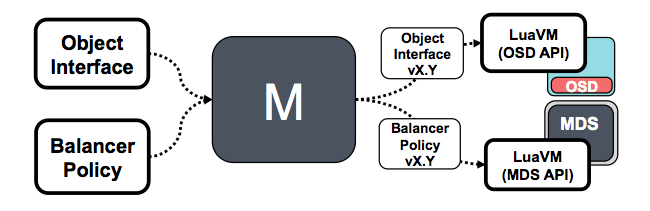
\includegraphics{figures/implementation.png}
\caption{Malacology re-uses Ceph subsystems to allow users to dynamically define 
new object interfaces and load balancing policies. It achieves this by extending 
the OSD and MDS subsystems with an embedded Lua VM. To manage newly dynamic 
interface classes, it exposes the core functionality of the Monitor to allow 
arbitrary data to be associated to ODS and MDS cluster maps. After new 
interfaces are submitted to the monitor and the associated Paxos proposal is 
accepted by the monitor quorum, the script is redundantly and consistently 
distributed to OSDs so this snippets persist.
\label{fig:implementation}}
\end{figure}

\paragraph*{Malacology:} The implementation of Ceph's object abstraction,
although powerful, has some drawbacks. Supporting only C/C++ for object
interface developers, Ceph requires distribution of compiled binaries for the
correct architecture, adding a large barrier of entry for developers and
system administrators. Second, having no way to dynamically unload modules,
any changes require a full restart of an OSD which may have serious
performance impacts due to a loss of cached data. And
finally, the security limitations of the framework limit the use of object
classes to all but those with administrative level access and deep technical
expertise.

To address these concerns, Malacology takes advantage of community contributed
Lua extensions to Ceph allowing new object interfaces to be dynamically loaded
into the system and modified at runtime, resulting in a object storage API
with economy of expression, which at the same time provides the full set of
features of the base object class. New object interfaces that are
expressed in thousands of lines of code can be implemented in approximately an
order of magnitude less code~\cite{geambasu_comet_2010}.

{\bf Interface management.} All of these modifications work in tandem to
implement the desired behavior, and are typically co-designed together such
that each depends on the other to behave as expected. In highly dynamic
environments such as a distributed storage system, changes to the system
propagate at variable rates, requiring all components of the system to be able
to adapt. Thus, system services realized through extensibility should be
versioned together as a group, exposing the version to allow introspection and
domain-specific treatment of version mismatch scenarios.

And finally, it is important to not underestimate the importance of the
preservation of the modifications that enable a new system service. In many
(if not all) cases, interfaces defining access to data are just as important
as the data itself by virtue of inherently providing structural context. Thus,
all components of a system service must be kept to the same standards of
protection as data in the system itself.

To this end we have extended the monitoring service using the framework
described in Section~\ref{sec:mon} to provide an interface for registration
and verification of dynamically defined object interfaces. Using this service
guarantees that interface definitions are not only made durable, but are
transparently and consistently propagated throughput the cluster and that
clients are properly synchronized with the latest interfaces.

\subsection{Distributed Metadata Services}
\label{malacology:mds}

The distributed metadata service in Ceph provides clients with a POSIX file
system abstraction~\cite{weil:sc2004-dyn-metadata}. In general, distributed
file systems protect resources by providing hierarchical indexing and
distributed locking services.  In Ceph, the locking service implements a
capability-based system that express what data and metadata clients are allowed
to access as well as what state they may cache and modify locally. While
designed for a fixed file abstraction, indexing, locking, and caching are all
common services that are useful to a broad spectrum of applications.

Ceph also addresses the challenge of balancing metadata load using load
balancing policies that compute metrics based on system state (e.g.  CPU and
memory utilization) and statistics collected by the cluster (e.g. the
popularity of an inode). Ceph uses dynamic subtree partitioning to move
variable sized namespace subtrees. These units can be shipped anywhere (i.e.,
to any MDS of any capacity) at any time for any reason. The original balancer
was designed with hard-coded policies and tunables.  Distributed applications
that share centralized resources (e.g. a database or directory) face similar
challenges which are often solved using application-specific sharding. 

%The metadata cluster moves units of the namespace called directory fragments
%and assigns them to servers using its own metadata load balancer. It then uses
%a hard-coded policy to balance these fragments using a scalarized load metric
%based on CPU, workload, and file system operation metrics. Although the CephFS
%balancer has been shown to be complicated, its complexity is justifiable.
%Having the flexibility to choose what to move, where to move it, and how much
%to move is very powerful. The problem is that it is difficult to pick a
%one-size-fits-all policy, system administrators may want to partition load
%based on SLAs, or applications are better equipped to make these decisions,
%etc. -- but we choose instead to expose a balancing API at strategic points in
%the balancing logic using Lua hooks. ~\cite{sevilla:sc15-mantle}. 

\paragraph*{Malacology:} New interface hooks are added in strategic spots in
the metadata service to control load balancing and capabilities, and for
defining new file types allowing the indexing service to be re-purposed for
other types of named resources.

{\bf Load balancing.} Mantle~\cite{sevilla:sc15-mantle}, a programmable
metadata load balancer, has been re-implemented on Malacology so that its
infrastructure can enjoy all the properties of other Ceph components. The load
balancing logic has stayed largely the same but the infrastructure has been
improved to safely load, manage, and persist its load balancing policies. 

{\bf Safely Loading Classes.} The original Mantle API is fragile: the API is
not enforced by the runtime, the system allows strings to be injected through the
admin daemon, constructing the Lua script in C++ is clunky, and the
administrator can inject really bad policies (e.g., while 1) that brings the
whole system down. Malacology exposes the important subsystems of Ceph's
logical storage device framework so that the MDS can safely and dynamically
load policies specified as Lua classes.

{\bf Policy management.} A new interface is added to the metadata service
subsystem using the monitoring framework to support management of interfaces. This 
ensures that the correct balancer version is consistently distributed and verified on
all MDS nodes. Policies are also durably saved with Ceph's replication and redundancy.

%These problems are general, distributed systems load balancing problems and
%share many of the same properties as the POSIX metadata
%wall~\cite{alam:pdsw2011-metadata-scaling,ghemawat:sosp2003-gfs,hildebrand:msst2005-pnfs,weil_ceph_2006,welch:fast2008-panasas,shvachko:login2012-hdfs-scalability}.
%Many distributed file systems decouple metadata and data I/O so that these
%services can scale independently. Despite this optimization, scaling the
%metadata services is still difficult because metadata accesses impose small
%and frequent requests on the underlying storage
%system~\cite{roselli:atec2000-FS-workloads}. Many techniques for designing the
%metadata services have been proposed to accommodate this workload:
%Lustre~\cite{konstantinos:pdsw2014-lustre-metadata},
%GFS~\cite{ghemawat:sosp2003-gfs}, and
%HDFS~\cite{shvachko:login2012-hdfs-scalability} keep all metadata on one
%server; GIGA+~\cite{patil:fast2011-giga}, IndexFS~\cite{ren:sc2014-indexfs},
%Lazy Hybrid~\cite{brandt:msst2003-lh}, GPFS~\cite{schmuck:fast2002-gpfs}, and
%pNFS~\cite{hildebrand:supercomputing2006-pNFS} hash the file system namespace
%across a dedicated cluster and cache metadata;
%Panasas~\cite{welch:fast2008-panasas} and
%CephFS~\cite{weil:sc2004-dyn-metadata} use subtree partitioning to carve up
%the namespace and distribute it across a cluster.
%
%Both the object and balancer interfaces define functions and attach them
%to the core Lua sandbox. For example, the Lua object storage interface
%class attaches data, extended attribute, object map, and object version
%functions, to the Lua core functions, as shown in Figure
%\ref{fig:cls-osd-mds}. The advantages of this is that we avoid
%duplicating code, we provide a framework for putting Lua code in other
%parts of the system, and we remove components and APIs that are too
%integrated with the OSD.

%To facilitate the use of Lua in both the MDS and OSD, we modularize the LuaVM
%in a core sandbox wrapper and link against it, as shown in
%Figure~\ref{fig:cls-osd-mds}. This core Lua wrapper contains just the
%dependencies, symbols, and functions, needed to run the Lua VM and strips away
%all the functionality inherent to object classes (like placement group
%filters, cryptography functions, object metadata,  object data, object
%extended attributes, and object versions). Some functions of Ceph's more
%helpful subsystems, like the logging facilities for the daemons, were re-used
%in the MDS.  With this scheme, The OSD will dynamically open the shared
%library created by Lua object interface shared library while the MDS will
%dynamically open the Lua balancer interface shared library; both shared
%libraries will the Lua core.

{\bf Capabilities.} The metadata service also manages sessions with its
clients. This gives both subsystems (MDSs and clients) the ability to cache
data and grab locks. The metadata service is responsible for responding to
client requests for capabilities by first revoking caps from other clients.
Currently, clients voluntarily release their capabilities, and the MDS maintains
a queue of requests.  Both clients and MDSs use a best-effort approach to
revoking or releasing capabilities.

The clients retain the best-effort, voluntary release of capabilities, but in
Malacology, the queuing policies are generalized within the MDS to allow for
centralized policies such as fairness or priority.

{\bf File Types.} We leverage the same active and typed storage module
presented in DataMods~\cite{watkins_datamods_2012} to assign state and a set of
functions to a file (stored in the inode). This is valuable for
metadata load balancing so that certain types of files can have a higher
priority when making balancing decisions.

%\begin{figure}[h]
%\centering
%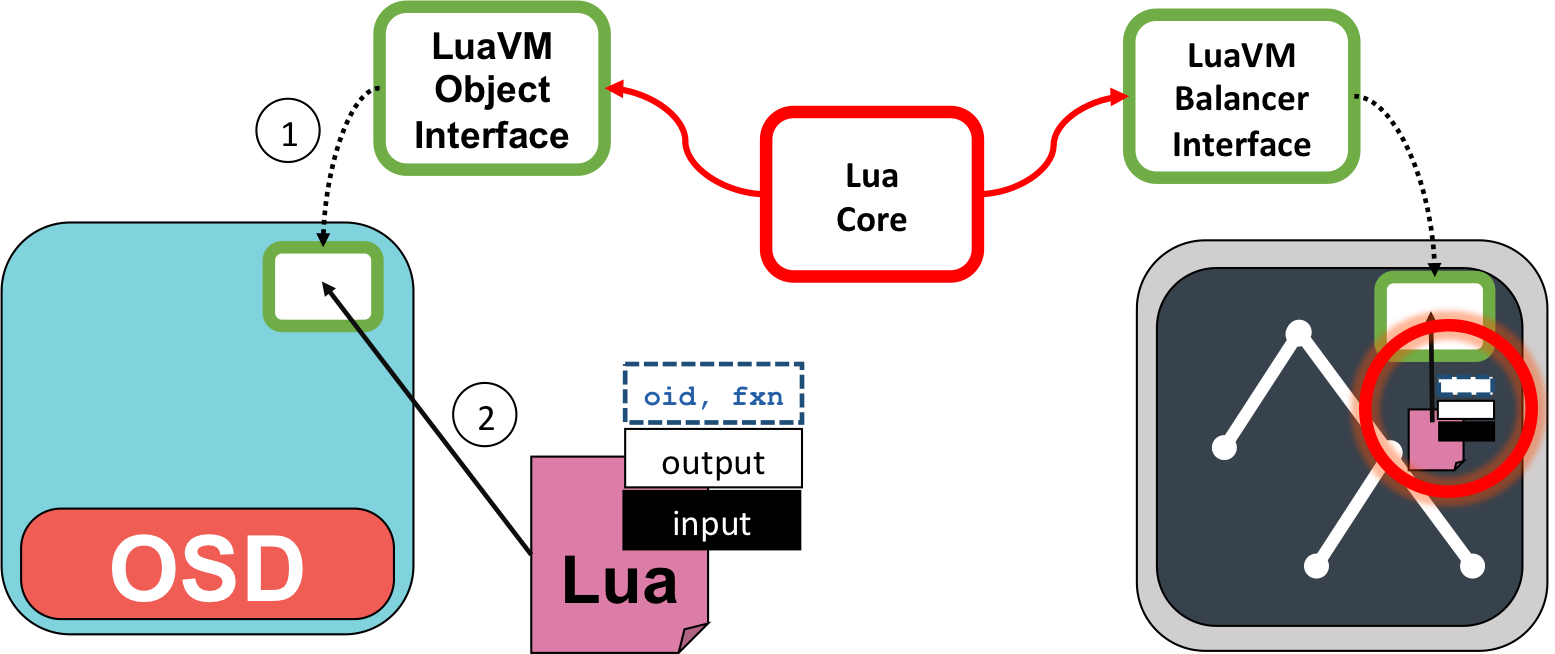
\includegraphics{figures/cls-osd-mds.png}
%\caption{To generalize the LuaVM for use in both the OSD and MDS,
%Malacology detaches the core functionality into a Lua core module. The
%VM is dynamically loaded first (1) and then interfaces can execute (2).
%\label{fig:cls-osd-mds}}
%\end{figure}

% Straw man example
%Migrating resources is an important part of load balancing but understanding
%the effects of different configurations and parameters is difficult. Systems
%already virtualize and migrate memory; soon systems will be able to migrate
%other resources, like CPU, disk, and memory. Figuring out how, when, and where
%to move these resources depends on complex metrics like utilization,
%configuration, and workload.

%These hooks embed Lua code in the MDS using the OSD subsystems. By re-using
%the OSD interface classes, the MDS gets the safety and robustness of loading
%dynamic code (including graceful failures and helpful errors), the ease of
%transferring state between object interfaces and the OSD internals,
%integration with testing and correctness suites, and \texttt{struct}s for
%interface data and handlers. 

\subsection{Durability}
\label{sec:durability}

Ceph provides storage by striping and replicating data across
RADOS~\cite{weil_rados_2007}, the reliable distributed object store. RADOS
uses many techniques to ensure that data is not corrupted or lost, such as
erasure coding, replication, and data scrubbing. Furthermore, many of these
techniques try to be autonomous so that work is distributed across the
cluster. For example, when placement groups change, the OSDs re-balance and
re-shard data in the background in a process called placement group splitting.

In order to reduce load on the monitoring service, Ceph OSDs use a gossip
protocol to efficiently propagate changes to cluster maps throughout the
system, and autonomously initiate recovery mechanisms when failures are
discovered.

\paragraph*{Malacology:} Metadata service policies and object storage interfaces are stored durability
within RADOS and managed by storing references with the object maps. Since
the cluster already propagates a consistent view of these data structures,
we use this service to automatically install interfaces in OSDs, and install
policies within the MDS such that clients and daemons are synchronized on
correct implementations without restarting.

\section{Services Built on Malacology}
\label{sec:services}
\label{services-built-on-malacology}

\label{services}

\begin{table}
\centering
\begin{tabular}{  l | l | l    }
\textbf{Service} & \textbf{Ceph Component} & \textbf{Used for...}  \\ \hline
Mantle  & RADOS    & policy durability \\
        & MON maps & policy versioning \\ \hline
ZLog    & Logical Storage & CORFU protocol  \\ 
        & MON maps & interface install \\ \hline
Seq.    & MDS file types & log management \\ 
        & MDS fault toler. & seq. fault toler. \\
\end{tabular}
\caption{To implement the Mantle and ZLog services, we leverage Ceph components. Malacology uses these subsystems because they provide powerful abstractions.}
\label{table:implementation}
\end{table}

In this section we describe two services built on top of Malacology. The first
is Mantle, a framework for dynamically specifying metadata load balancing
policies. The second system, ZLog, is a high-performance distributed shared-log.
In addition to these services, we'll demonstrate how we combine ZLog and Mantle
to implement service-aware metadata load balancing policies.

\subsection{Mantle: A Programmable Metadata Load Balancer}
\label{sec:mantle}

Mantle is a programmable metadata
balancer for Ceph that separates the metadata balancing policies from their
mechanisms. Administrators inject code to change how the metadata cluster
distributes metadata. In ~\cite{sevilla:sc15-mantle} the authors showed how 
using Mantle, one can implement a single node metadata service, a distributed 
metadata services with hashing, and a distributed metadata service with dynamic 
subtree partitioning.

\subsection{Re-Implementation}

The Ceph team wants to merge Mantle because the scriptability is useful for
debugging, controlling the metadata balancer, and examining trade-offs for
different balancers. Unfortunately, this research quality system is not as
robust as Ceph and the Ceph team wants more safety, durability, and consistency
for the new services.  The API for Malacology is the same as the one exposed
in~\cite{sevilla:sc15-mantle} but the hooks are put in different places.

\subsection{Policy Versioning}

For Mantle, we added new monitor command to change the metadata load balancers:

\noindent \texttt{ mds\ set\ lua\_balancer\_class\ \textless{}version\textgreater{}}
%\noindent \texttt{ceph\ osd\ pool\ set-class\ \textless{}pool\textgreater{}\ \textless{}class\textgreater{}\ \textless{}script\textgreater{}}

This command assigns the current version of the metadata load balancer. In our case, it is simply the name of the balancer. The MONs take the version and store it in the MDS map. Similar to the PG map or MON maps, the MDS map has all the information about the topology and state of the MDS cluster. Leveraging the MONs helps ease the burden on the MDS to propagate the policy and ensure that everyone agrees.

There are Ceph components that are obstacles to this approach, namely the size of the  MDS map, API changes, and security. The Ceph engineers want to avoid using the maps to exchange information; the maps should be lightweight and fast because the MONs need to be able to version MDS cluster state quickly. API changes can also be a burden, especially for the MDS map, since all clients need to have the same version of the CephFS library in order to properly interact with CephFS. Finally, Ceph tries to avoid injecting strings into the cluster because they are insecure and buggy. 

\subsection{Making Policies Durable}

While storing the code snippets that define the policies in the MDS map is 
possible, it is not recommended as it is an expensive operation (a PAXOS voting 
round). Thus, Malacology only stores policies IDs which correspond to an object 
in a system-maintained pool. When MDSs read a policy, they first check latest 
version from the MDS map, and then dereference the pointer by reading the 
corresponding object in RADOS.

\subsection{ZLog: A Fast Distributed Shared-Log}
\label{sec:zlog}

The second service implemented on Malacology is ZLog, a high-performance
distributed shared-log that is based on the CORFU
protocol~\cite{balakrishnan_corfu_2012}. A
shared-log is a general, yet powerful abstraction used to build many
distributed systems. However, existing implementations that rely on consensus
algorithms such as PAXOS funnel I/O through a single point introducing a
bottleneck that restricts throughput. In contrast, the CORFU protocol is able
to achieve high throughput using a network counter service, called a 
\emph{sequencer}, that avoids all persistent I/O in the common case.

While a full description of the CORFU system is beyond the scope of this
paper, we'll briefly describe the custom storage device interface, sequencer
service, and recovery protocol, and how these services are instantiated in the
Malacology framework.

\subsubsection{Sequencer}

High-performance in CORFU is achieved using a sequencer service that assigns
log positions to clients by reading from a volatile, in-memory counter which
can run at a very high throughput and at low-latency. And since the sequencer
is centralized, ensuring serializability in the common case is trivial.  The
primary challenge in CORFU is handling the failure of the sequencer in a way
that preserves correctness. Failure of the sequencer service in CORFU is
handled by a recovery algorithm that recomputes the new sequencer state using
an application-specific custom storage interface to discover the tail of the
log, while simultaneously invalidating stale client requests using an
epoch-based protocol.

We implement the sequencer service in Malacology as an application-specific
file type that associates a small amount of metadata, including the 64-bit log
tail position, to the inode state managed by the Ceph metadata service. Since
a sequencer is associated with a unique log, this approach has the added
benefit of allowing the metadata service to also handle naming, by
representing each log service instance within the standard POSIX hierarchical
namespace.

{\bf Sequencer interface.} The sequencer resource supports the ability to
\emph{read()} the current tail value as well get the \emph{next()} position in
the log which also atomically increments the tail position. We implement this
functionality as methods on ZLog inode resources. The primary challenge in
mapping the sequencer resource to the metadata service is handling
serialization correctly.

Initially we sought to directly model the sequencer service in Ceph as a
non-exclusive, non-cacheable resource, forcing clients to perform a round-trip
access to the resource at the authoritative metadata server for the sequencer
inode.  Interestingly, we found that the capability system in Ceph uses a
strategy to reduce metadata service load by allowing multiple clients that
open a shared file to temporarily cache the inode resource, resulting in a
round-robin, best-effort batching behavior. When a single client is accessing
the sequencer resource it is able to cache state locally without interruption.

While unexpected, this discovery allowed us to explore an implementation
strategy that we had not previously considered. In particular, for bursty
clients, and clients that can tolerate increased latency, this mode of operation may
allow a system to achieve much higher throughput than a system with a
centralized sequencer service.
We utilize the programmability of the metadata service to define a new policy
for handling capabilities that controls the amount of time that clients are
able to cache the sequencer resource. This allows an administrator or
application to control the trade-off between latency and throughput beyond the
standard best-effort policy that is present in Ceph by default.

In Section~\ref{evaluation} we quantify the trade-offs of throughput and
latency for an approach based on a round-robin batching mode, and compare this
mode to one in which the metadata server mediates access to the sequencer
state when in it is being shared among multiple clients.

{\bf Balancing policies.}
As opposed to the batching mode for controlling access to the sequencer
resource, more predictable latency can be achieved by treating the sequencer
inode as a shared non-cacheable resource, forcing clients to make a round-trip
to the metadata service. However, the shared nature of the metadata service
may prevent the sequencer from achieving maximum throughput. To provide a
solution to this issue we have taken advantage of the programmability of the
metadata service load balancing to construct a service-specific load balancing
policy. As opposed to a generic balancing policy that may strive for uniform
load distribution, a ZLog-specific policy may utilize knowledge of inode types
to migrate the sequencer service to provisioned hardware during periods of
contention or high demand.

\subsubsection{Storage Interface}

The storage interface is a critical component in the CORFU design. Clients
independently map log positions that they have obtained from a sequencer
service (described in detail in the next section) onto storage devices, while
storage devices provide an intelligent \emph{write}-once, random \emph{read}
interface for accessing log entries. The key to correctness in CORFU lies with
the enforcement of up-to-date epoch tags on client requests; requests tagged
with out-of-date epoch values are rejected, and clients are expected to
request a new tail from the sequencer after refreshing state from an auxiliary
service.  This mechanism forms the basis for sequencer recovery.

In order to repopulate the cached tail value during recovery of a sequencer,
the maximum position in the log must be obtained. To do this, the storage
interface exposes an additional \emph{seal} method that atomically installs a
new epoch value and returns the maximum log position that has been written.
Since the recovery protocol does not inform clients of a new epoch value until
the end of the process, the validity of the tail can be guaranteed despite the
iterative process of contacting storage devices.  Recovery of the sequencer
process itself may be handled in many ways, such as leader election using an
auxiliary service such as PAXOS.

\section{Evaluation}
\label{evaluation}
We have conducted our evaluation on CloudLab as well as our own 20 node cluster. We follow the ``Popper Convention"~\cite{anonymous} so as to try and make our experiments as reproducible as possible. We have a GitHub repository with our source code,  experimental environment, configuration parameters, and workloads in a GitHub repository. Due to the double-blind policy, we have temporarily disabled the links to our graphs and experimental details.

Much of this work focuses on the programmability of Ceph and the services that
can be layered on top of Malacology. As such, we focus on the performance of the 
components and subsystems exposed by the framework. Detailed system-wide performance
measurements and analysis is forthcoming for both Mantle and ZLog~\cite{}, as we try
to find the best metadata balancing policies and physical design implementation trade-offs
respectively.

\subsection{ZLog}

We evaluate the mapping of ZLog onto Malacology by examining the costs of
utilizing the metadata service as a sequencer, and propagating interface
changes throughout the cluster using the monitoring service. We have omitted
evaluation of the overhead costs of adding object interfaces themselves due to
lack of space, and the fact that they are heavily tested and used already in
production with acceptable performance, introducing a small constant overhead
per operation but otherwise does not affect scalability.

\subsubsection{Sequencer}

We evaluated the performance of the ZLog Sequencer implemented in several
different configurations by showing a trade-off between aggregate throughput
achieved (shown in Figure~\ref{fig:captp}), and latency distribution (shown in
Figure~\ref{fig:capcdf}).

In Figure~\ref{fig:captp} the highest throughput labeled $1C$ shows that a
single client caching the sequencer resource may obtain new sequences at a rate
of nearly 6 million positions per second. This is not surprising given that all
state is cached locally in the client. When this resource is shared between two
clients, the MDS uses a best-effort approach to granting the sequencer resource
to each client (value $2C,BE$). This sharing has a large impact on performance,
as shown by the nearly three orders of magnitude drop off in throughput.

\begin{figure}[h]
\centering
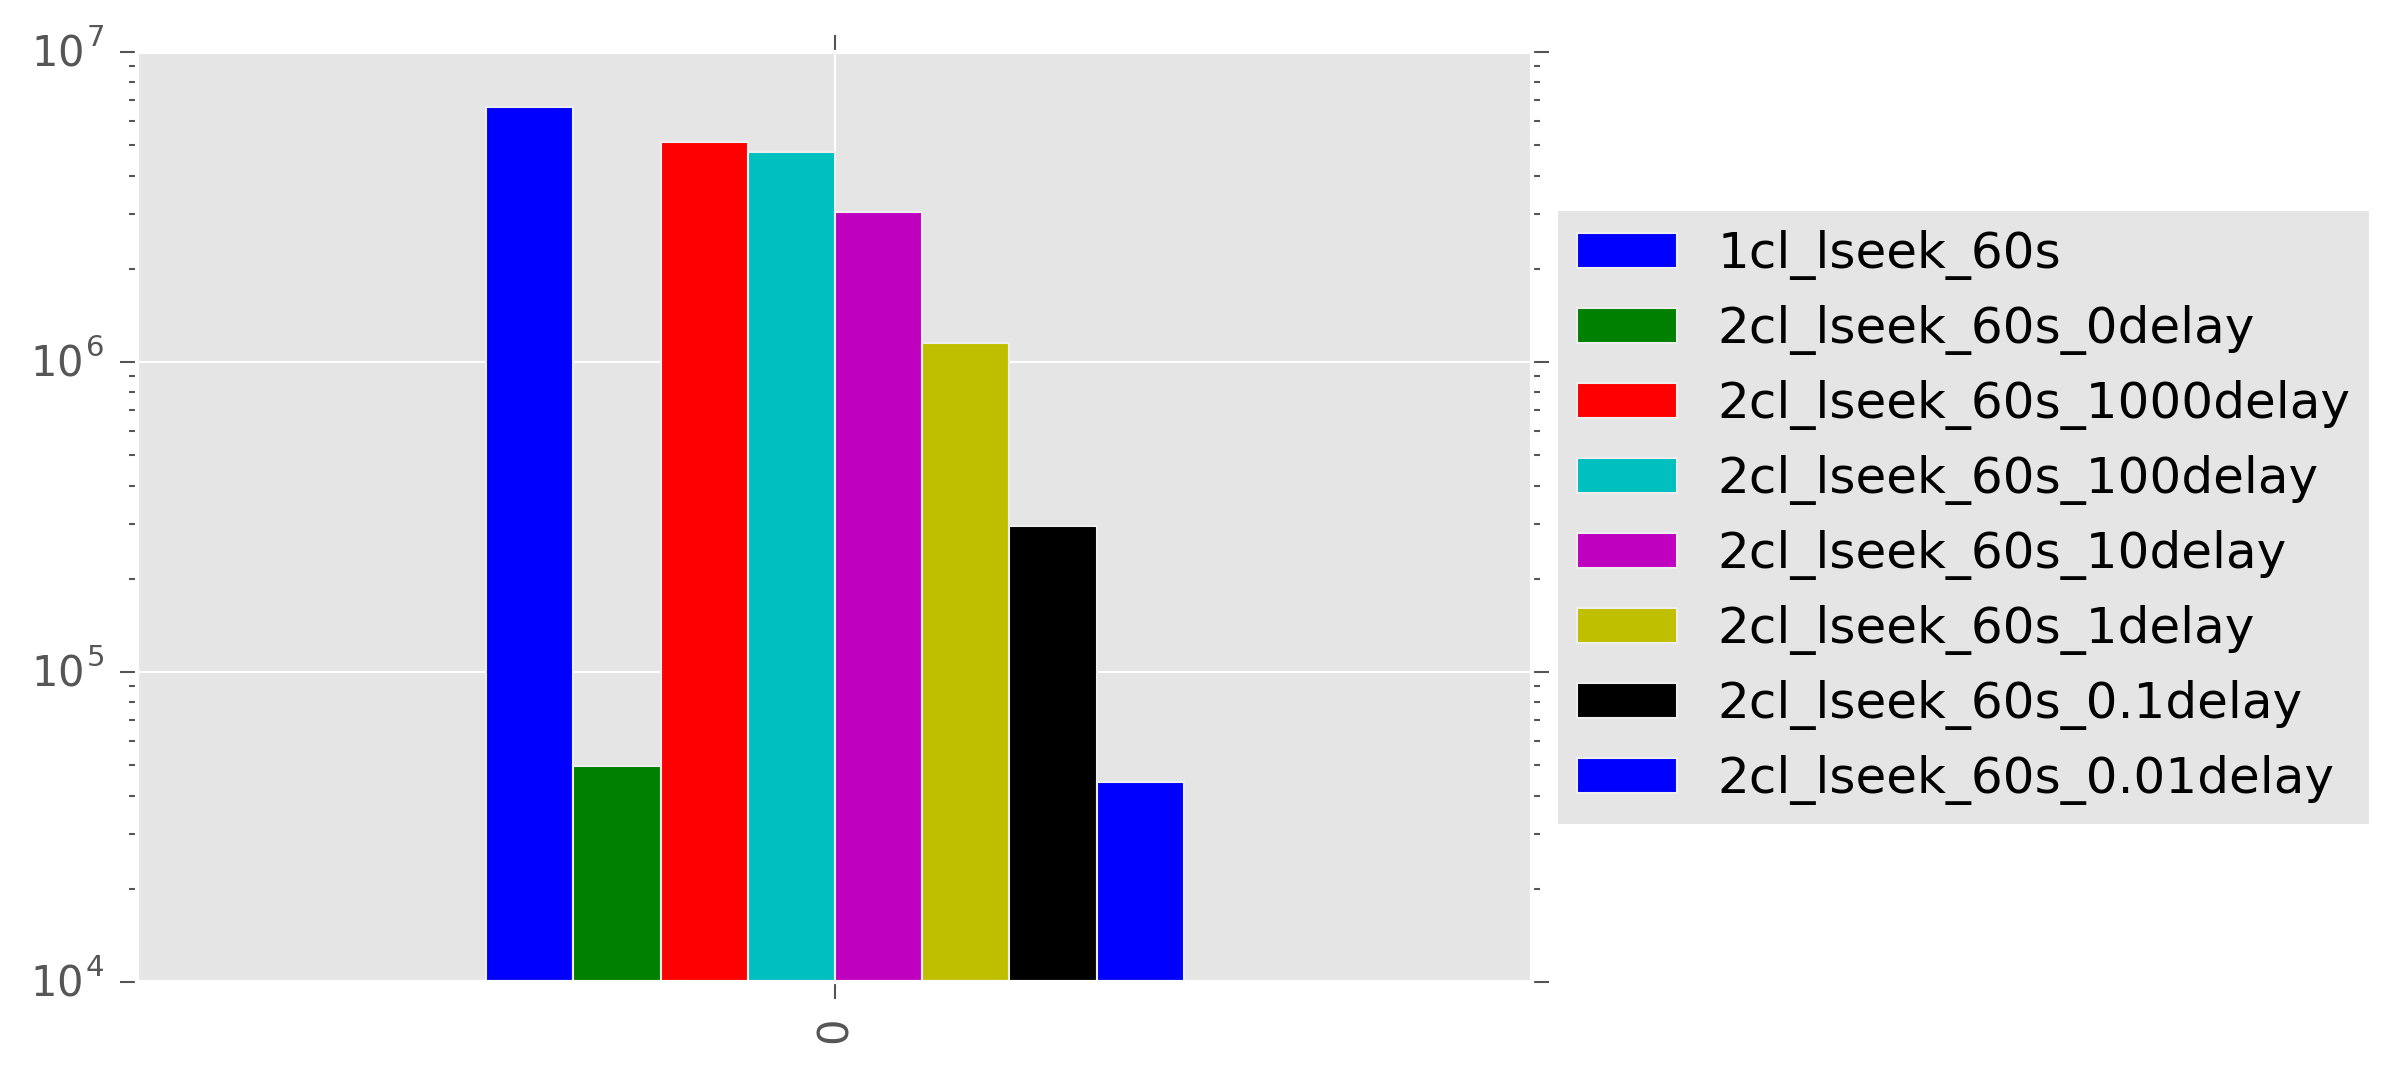
\includegraphics{figures/caps-delay-thruput.png}
\caption{Sequencer throughput by reusing various services.
The highest performance is achieved using a single client with
exclusive, cacheable privilege. Round-robin sharing of the sequencer
resource is affected by the amount of time the resource is held,
with best-effort performing the worst.}
\label{fig:captp}
\end{figure}

\begin{figure}[h]
\centering
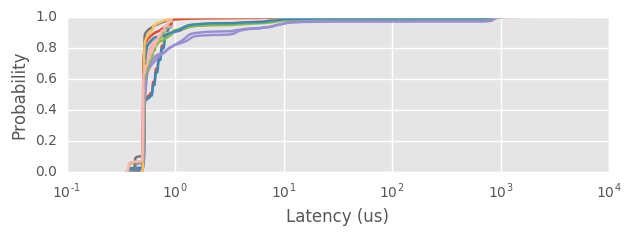
\includegraphics{figures/caps-delay-latency.png}
\caption{But if the clients hold their capabilities longer, it hurts
latency for everyone.}
\label{fig:capcdf}
\end{figure}

While a best-effort approach to sharing capabilities makes sense for a file
system client, throughput drops significantly with two clients as the majority
of the time neither client has the capability as it ping-pongs between
clients. This observation reveals a tuning parameter: how long a client
maintains its capability lease. In throughput labeled $2C,<time>$ we show
aggregate throughput as we decrease the amount of time that a client holds its
lease before responding to a request for the capability.  At lease times as
low as 10ms throughput achieve a significant proportion of the locally cached
throughput.

\textbf{The Malacology Approach:} Re-use the capability management features of the MDS.
While the batching mechanism can achieve high-throughput, it is not appropriate
for applications that require predictable latency. The throughput in
Figure~\ref{fig:captp} labeled $2C,ZLog$ corresponds to a centralized
sequencer implementation. While throughput is lower for two clients (because of
the synchronous network round-trip required for each request),
Figure~\ref{fig:capcdf} shows that this approach achieves more predicable
latency compared to all other approaches except for the single client locally
cached mode.


\subsubsection{Interface Propagation}

In Section~\ref{consistencyversioning-of-cluster-state} we described an
interface management service that is responsible for the durable and
consistent cluster-wide distribution of interface versions. We evaluate the
costs of such a service by embedding interface definitions in a Ceph cluster
membership data structure that is managed by a PAXOS instance, and distributed
using a scalable, peer-to-peer gossip protocol that is built into Ceph. We
assume an architecture that consists of a light-weight interface that enforces
the semantics of interface management resulting in one or more interface
updates that must be consistent across the cluster. The following experiments
focus on the cost of achieving distribution of consistent a interface version.

\begin{figure}[h]
\centering
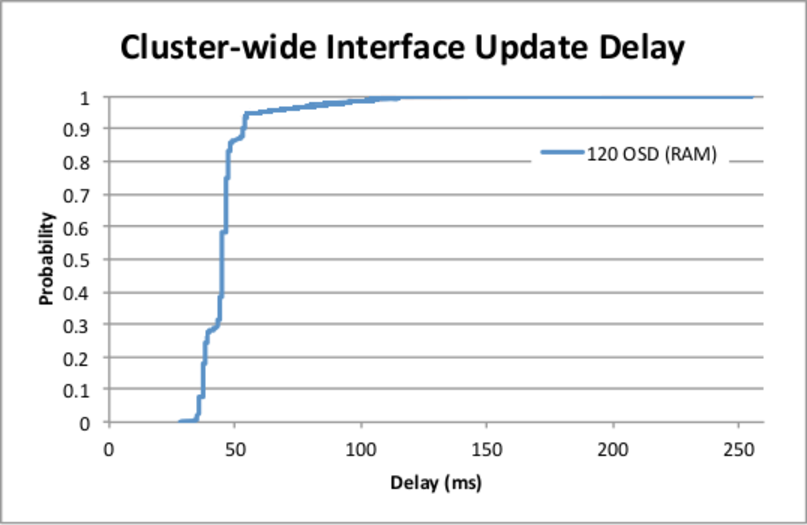
\includegraphics[trim={1 4 4 1.3cm},clip]{figures/iface-update-delay.pdf}
\caption{Cluster-wide interface update latency, excluding the Paxos proposal cost for
interface commit. Each of the 120 OSDs used a RAM-based object store, while the
3 OSDs used an HDD-backed object store.}
\label{fig:propdelay}
\end{figure}

Figure~\ref{fig:propdelay} shows the CDF of the latency of installing and
distributing an interface update on all OSDs in the cluster. The latency is
defined as the elapsed time following the PAXOS proposal for an interface
update until each OSD makes the update live (the cost of the PAXOS proposal is
configurable and is discussed below). The latency measurements were taken on
the nodes running Ceph server daemons, and thus exclude the client round-trip
cost. In each of the experiments 1000 interface updates were observed.

The first experiment shown in Figure~\ref{fig:propdelay} illustrates a lower
bound cost for updates in a large cluster by avoiding disk I/O for storing
interface updates locally within each OSD.  In the experiment labeled "120 OSD
(RAM)" a cluster of 120 OSDs (10 OSDs x 12 servers) using an in-memory data
store were deployed, showing a latency of less than 54 ms with a probability
of 90\% and a worst case latency of 194 ms. The curve labeled "3 OSD (HDD)" is
a smaller cluster where each of the three OSDs uses a spinning disk as the
object store that saves a copy of the cluster map, and shows a latency of 37
ms with a 90\% probability and a worst case latency of 255 ms. Since the cost
of a disk I/O is larger than the same I/O executed against the in-memory
device, the predominant cost in a lightly loaded cluster appears to be the
number of OSDs.

\textbf{The Malacology Approach:} Re-use Ceph's Monitor functionality to 
propagate application-specific state that needs to be highly-available and 
strongly consistent.
The real cost of interface management, in addition to cluster-wide propagation
of interface updates, includes the network round-trip to the interface
management service, the PAXOS commit protocol, and other factors such as system
load. By default PAXOS proposals occur periodically with a 1 second interval in
order to accumulate updates. In a minimum, realistic quorum of 3 monitors using
HDD-based storage, we were able to decrease this interval to an average of 222
ms.

\subsection{MDS as a ZLog Sequencer}

The following experiments demonstrate the feasibility of using the Ceph MDS
cluster as a sequencer. The goal of the workloads is to saturate the MDS
cluster, so we design sequencers uses a more heavy-weight file system
operation. The experiments use our internal cluster and there are 15 clients
and between 1 and 3 MDS nodes. 

\begin{figure}[t!]
\centering
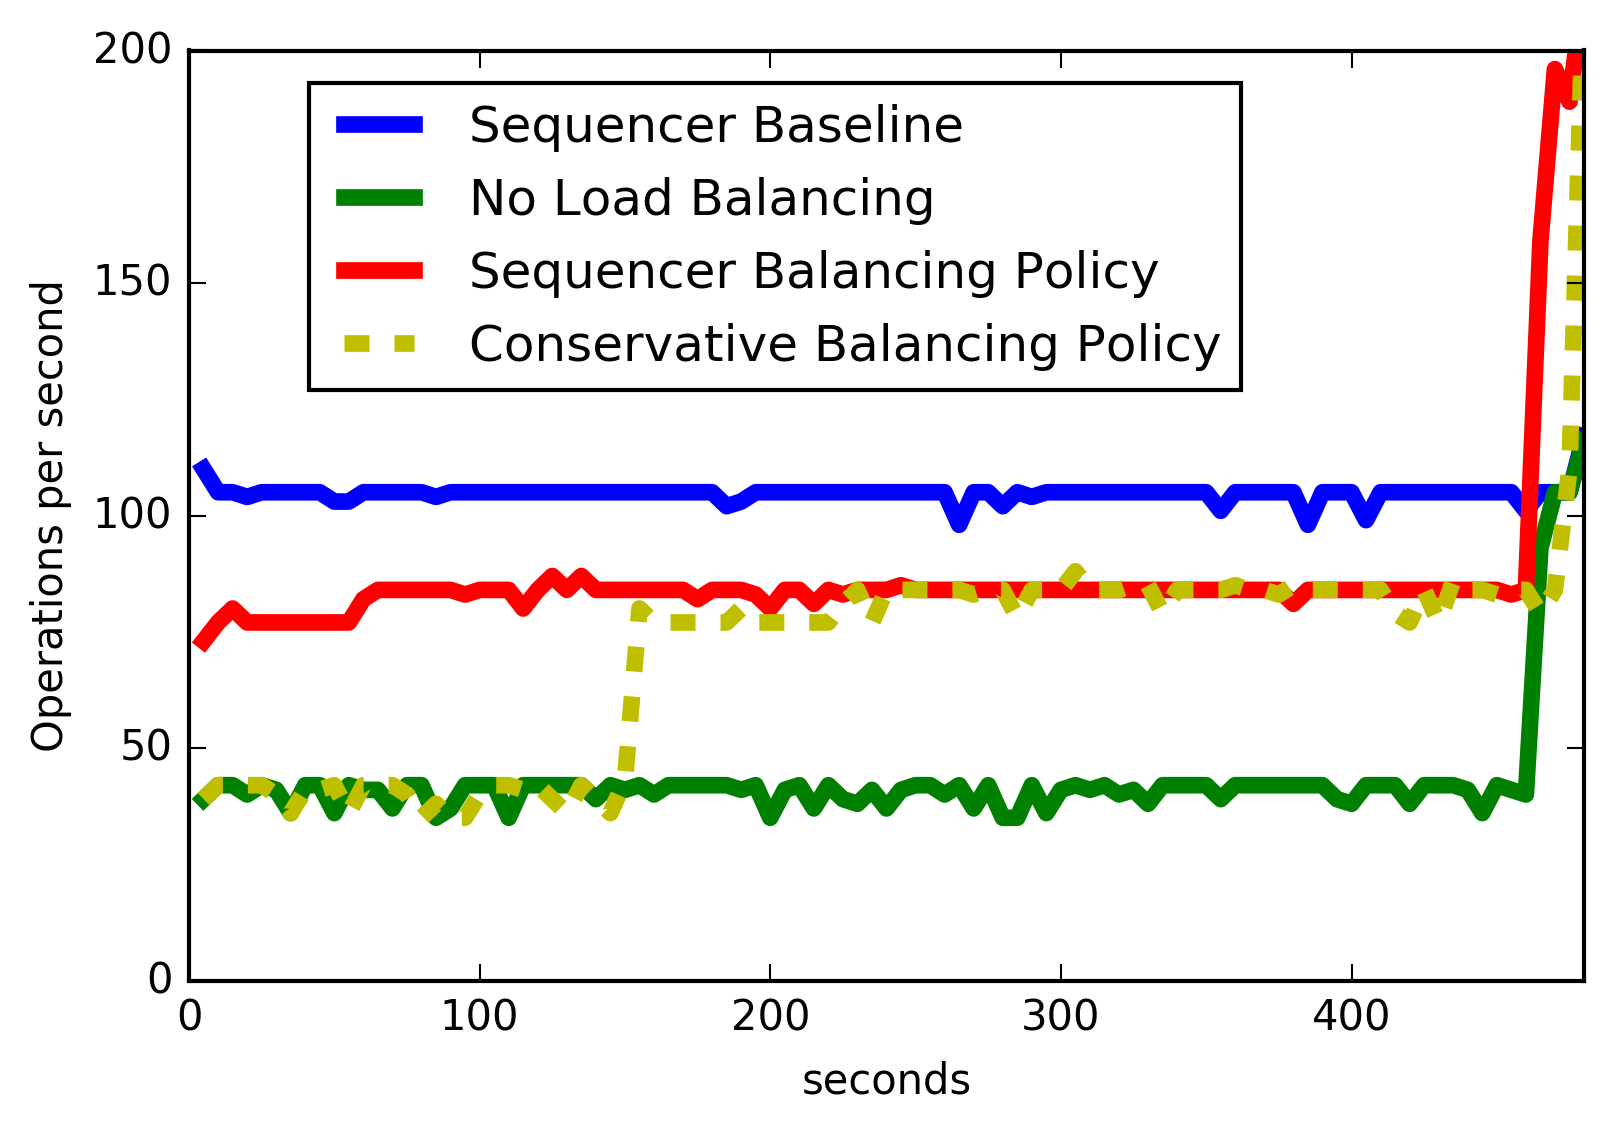
\includegraphics{figures/mantle-seq-thruput.png}
\caption{A ZLog sequencer that uses the CephFS MDS enjoys the load balancing
capabilities of the metadata cluster. The ``Sequencer Baseline'' has no
background sequencers, while the ``2 Seq'' curves are the throughput
of 1 sequencer when an additional sequencer is running in the background
generating load.}\label{fig:mantle-seq-thruput}
\end{figure}

\subsubsection{Load Balancing}

We use a balancer policy specifically designed for the sequencer. The balancer aggressively sheds half its load to its neighbor as soon as it can.  It is based
off the ``Greedy Spill Even" approach in the Mantle~\cite{sevilla:sc15-mantle} paper
but is reproduced here for the reader's convenience. 

\begin{figure}[]
\begin{lstlisting}
  -- Metadata server load
  mdsload = MDSs[i]["all"]
  
  -- When policy
  if MDSs[whoami]["load"]>.01 and 
    MDSs[whoami+1]["load"]<.01 then
    
  -- Where policy
  targets[whoami+1]=allmetaload/2
\end{lstlisting}
    \caption{The sequencer balancing policy that works best for bursty workloads. \label{listing:greedy-spill}}
\end{figure}

\begin{figure}[t!]
\centering
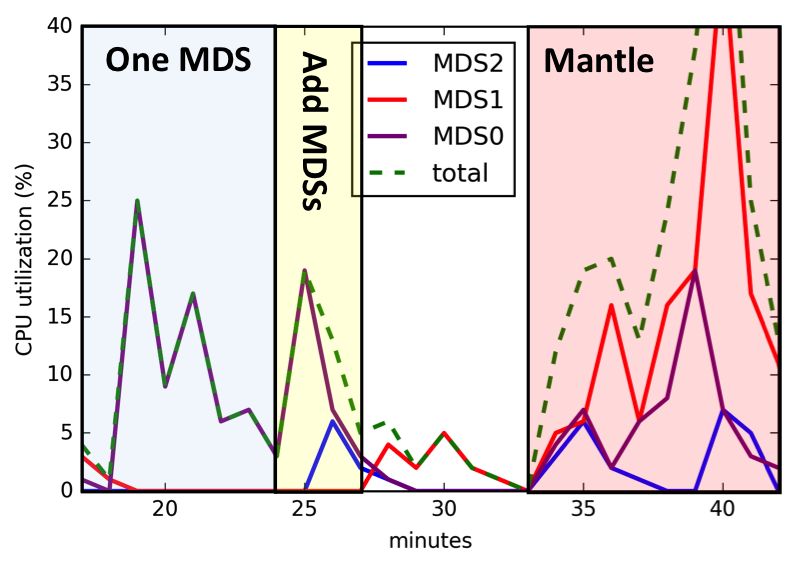
\includegraphics{figures/mantle-cpu-utilization-annotate.png}
\caption{The sequencer using Mantle in Figure~\ref{fig:mantle-seq-thruput}
migrates to a new MDS immediately because its uses a policy designed for bursty
workloads. This is a trace of the same workload running twice: once with a
single MDS and once with Mantle.}
\label{fig:mantle-cpu-utilization}
\end{figure}

Figure~\ref{fig:mantle-seq-thruput} gives a macro-level view of the performance
of the Ceph components exposed by Malacology. Each curve shows the throughput
from the perspective of one sequencer (\(y\) axis) over time (\(x\) axis).  The
``Sequencer Baseline'' curve is one sequencer serving 7 clients.  The sequencer
operates on an MDS cluster where balancing is turned off and there are no other
workloads running. ``No Load Balancing" adds another sequencer of equal load
running in the background. The performance of the background sequencer is
omitted. The last two policies, ``Sequencer Balancing Policy" and
``Conservative Balancing Policy", show the performance of the sequencer (with a
background sequencer running) when using Mantle with a 3 MDS node cluster.
These policies differ by the threshold at which they start balancing:
``Sequencer Balancing Policy" starts balancing immediately and ``Conservative
Balancing Policy" waits for 120 seconds.

Figure~\ref{fig:mantle-cpu-utilization} gives a time series graph to show the
behavior of the same workload, 2 sequencers, with balancing turned on and off.
The curves are the throughput (\(y\) axis) over time (\(x\) axis) and the graph
has been partitioned into the two cluster setups. The CPU utilization is
confined to one core the MDS is not multi-threaded, as it has been shown that
metadata performance does not improve with multiple
threads~\cite{konstantinos:pdsw2014-lustre-metadata}. 

Overall, the clients achieve lower performance than the capability experiments
in Figure~\ref{fig:captp} because the sequencer uses a slower metadata
operation to manage the capability.  ``Sequencer Baseline" is the best
performance for this particular workload because there is no contention.
Performance is stable and the MDS is under-loaded because we do not see the
spike at the end like the other curves. It appears the bottleneck is somewhere
with the clients -- perhaps it is our 1GBit/s network link. ``2 Seq; No Load
Balancing" shows an overloaded sequencer because the performance of our one
sequencer is low and unstable (high variation in performance). We also deduce
that it is overloaded by comparing to the ``2 Seq; Mantle Load Balancing"
curve, which shows improved performance when load is migrated. At 10 seconds,
the sequencer balancer immediately starts balancing and decides that two
sequencer streams should be split onto two MDSs. It migrates to its neighbor as
per the policy. 

\textbf{The Malacology Approach:} Re-use the Ceph metadata migration, load
balancing, cache coherence, and capabilities subsystems of the MDS. Applying
Mantle's load balancing policy shows 2.02\(\times\) performance improvement and
16\% degradation in performance over the baseline, even though the baseline has
half as many clients.

\subsubsection{Recovery}

\begin{figure}[t]
\centering
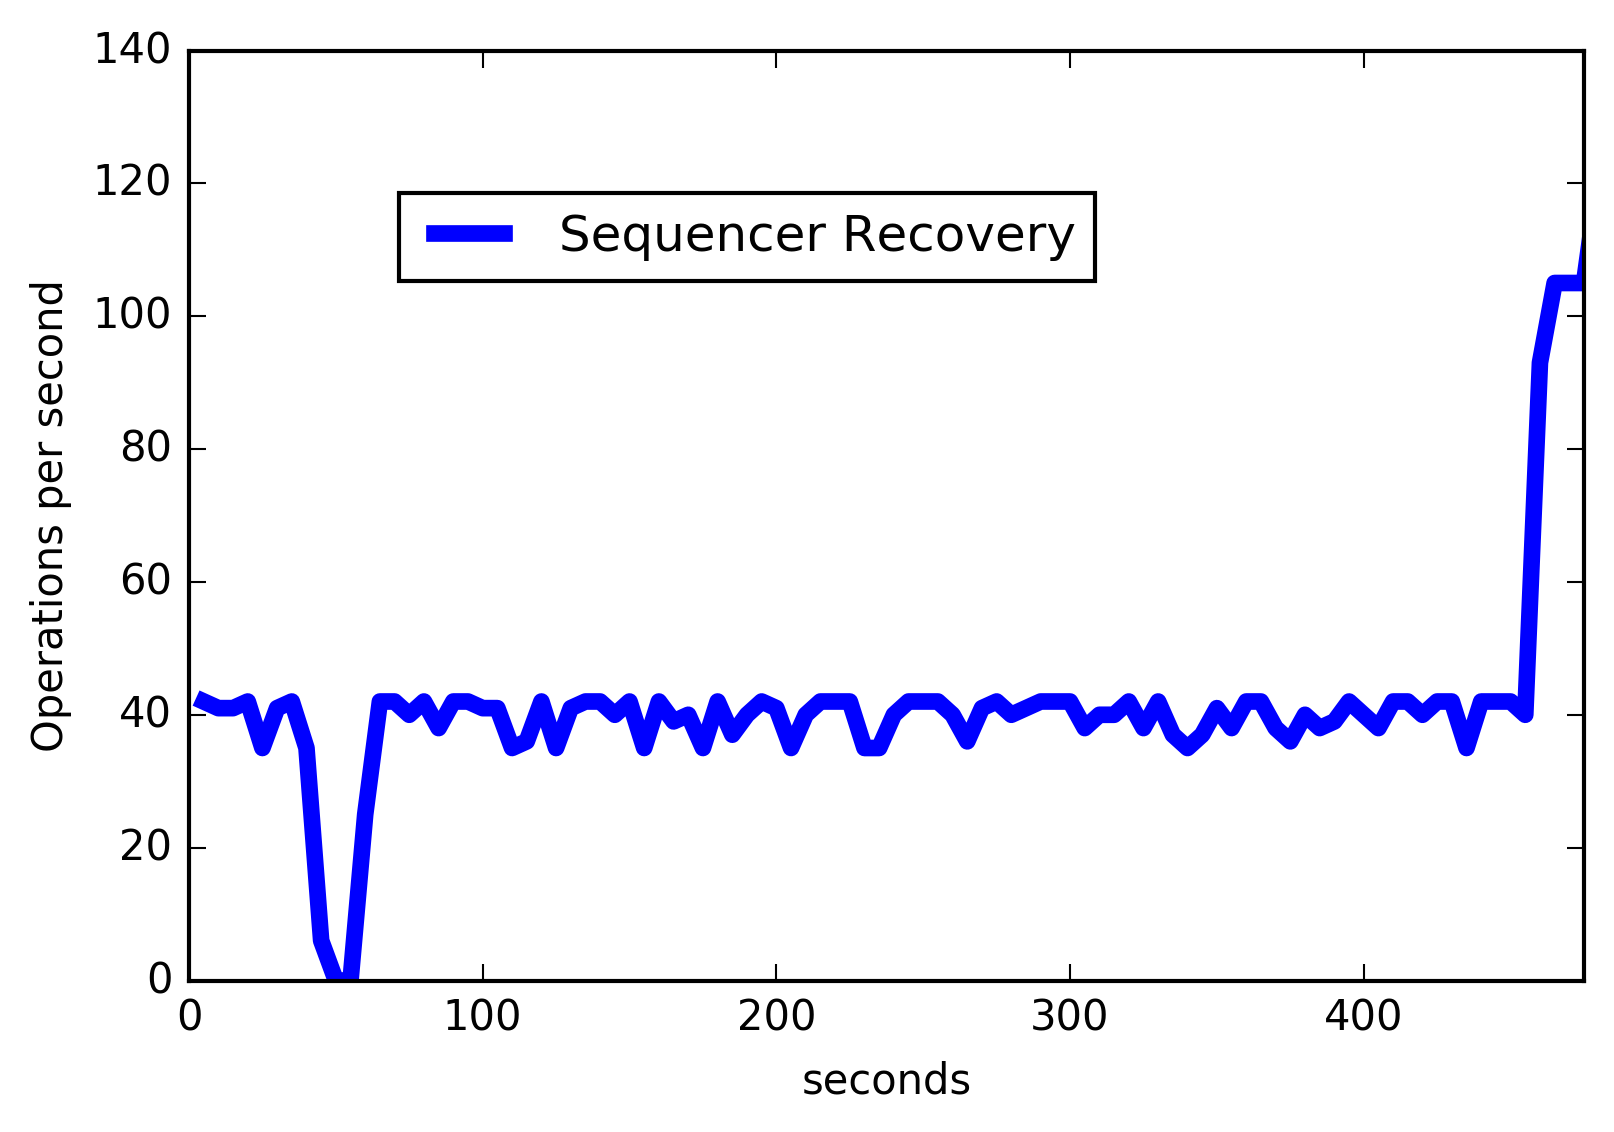
\includegraphics{figures/recovery-seq-thruput.png}
\caption{The sequencer using Mantle also inherits all the recovery protocols of
the Ceph metadata cluster. The throughput of the sequencer drops when we
terminal MDS 0. The performance quickly resumes and the sequencer is only down
for 15 seconds.}
\label{fig:recovery-seq-thruput}
\end{figure}

This experiment shows how a sequencer handing out tokens can use the Ceph MDS
recovery protocols to recover. For this workload, two sequencers are running on
a metadata cluster {\it without} multiple active MDS nodes. In this cluster,
MDS 1 and MDS 2 are in ``standby" mode, meaning one of them will step in should
the head MDS 0 fail. At the 60 second mark, we manually kill MDS 0. 

Figure~\ref{fig:recovery-seq-thruput} shows the sequencer throughput (\(y\)
axis) over time (\(x\) axis). When MDS 0 dies, the MON cluster notices and
quickly assigns a new MDS to handle the namespace. This is when MDS 1 takes
over the sequencer duties and starts handing out tokens.

\textbf{The Malacology Approach:} Re-use the Ceph metadata protocols for
failure detection and recovery. The sequencer recovers in 15 seconds on a new
MDS and it maintains the same throughput that it had before the failure.

%\subsubsection{Experiment: Object Class
%Programmability}\label{experiment-object-class-programmability}
%
%Add quote from CORFU paper that talks about what they had to hack
%
%\subsubsection{Experiment: Multi-Client
%Burstiness}\label{experiment-multi-client-burstiness}
%
%\begin{figure}[htbp]
%\centering
%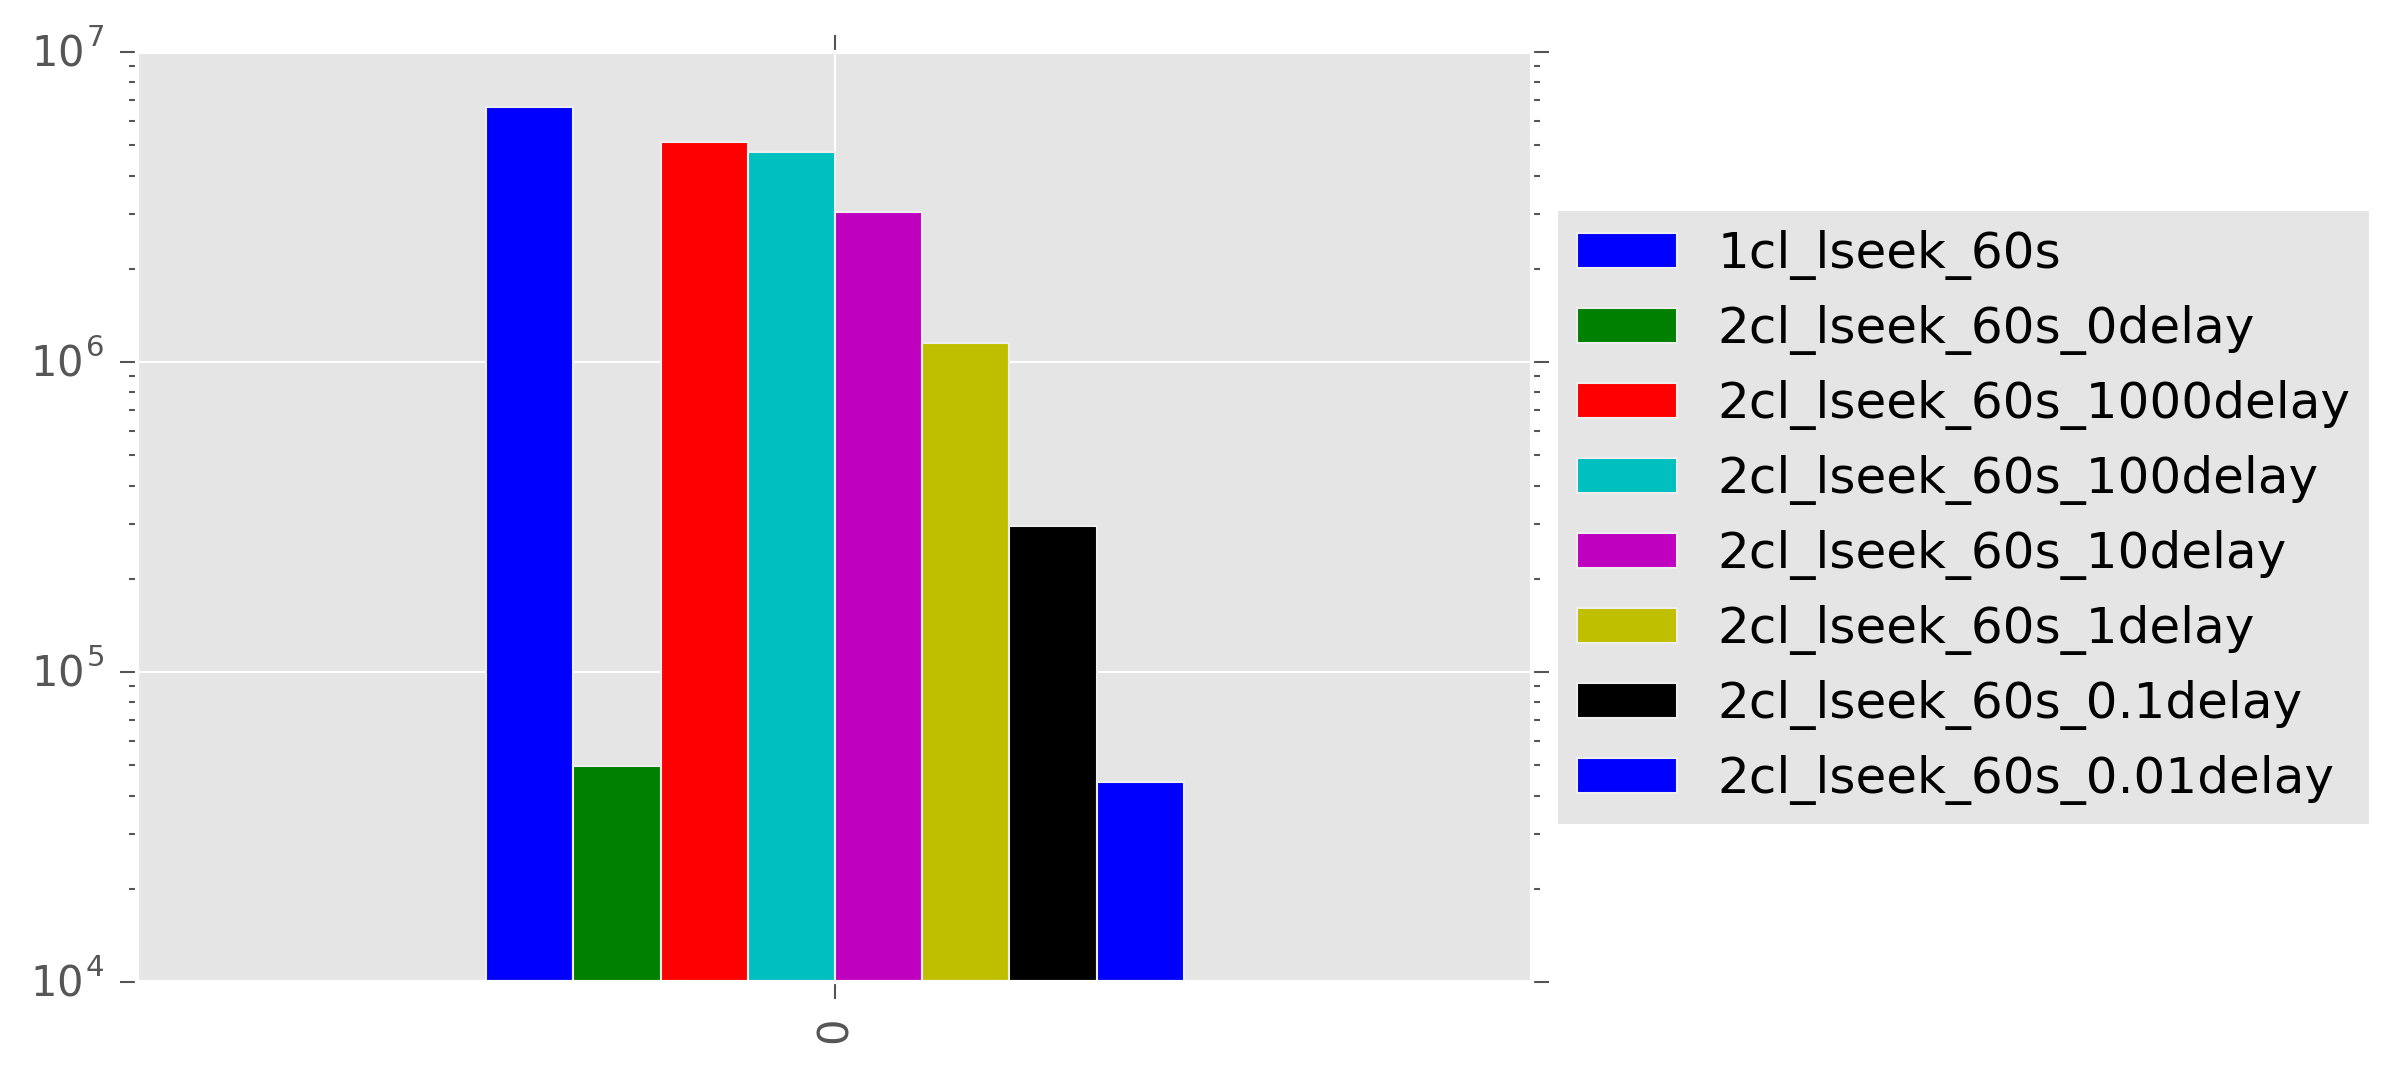
\includegraphics{figures/caps-delay-thruput.png}
%\caption{Forcing the client to drop their capabilities later (delay)
%improves throughput}
%\end{figure}

\section{Related Work}

% IOStack: Software-Defined Object Storage
% sRoute: Treating the Storage Stack Like a Network
   % - lots of good refs to check out
% Information and control in gray-box systems

Programmability of operating systems and networking resources, including distributed storage systems is not new, but we are not aware of work that makes generalization of existing services into programmable resourses a key principle in storage systems design. 

Programmable storage systems can be viewed as an infrastructure for creating abstractions to better separate policies from mechanisms. This idea is not new. Software-defined networks (SDNs) create such an abstraction by separating the control plane from the data plane (see for example~\cite{jain:sigcomm13}). This notion of control/data separation was also applied in software-defined storage (SDS)~\cite{arpaci:sosp01,thereska:sosp13,stefanovici:fast16}. Similarly, IOStack~\cite{gracia:internet16} is providing policy-based provisioning and filtering in OpenStack Swift. 

Another view of programmable storage systems is one of tailoring systems resources to applications~\cite{arpaci:sosp01}. Related work includes work around the Exokernel~\cite{engler:sosp95} and SPIN~\cite{bershad:sosp95} and Vino~\cite{seltzer:osdi96}, the latter two addressed the ability of injecting code into the kernel to specialize resource management. Another approach is to pass hints between the different layers of the IO stack to bridge the semantic gap between applications and storage~\cite{arpaci:sosp01,sivathanu:fast03,mesnier:sosp11}).

Malacology uses the same Active and Typed Storage module presented in
DataMods~\cite{watkins_datamods_2012}; Asynchronous Service and File
Manifolds can be implemented with small changes to the Malacology
framework, namely asynchronous object calls and Lua stubs in the inode,
respectively.

\section{Conclusion and Future Work}\label{conclusion-and-future-work}

Programmable storage is a viable method for eliminating duplication of
complex error prone software that are used as workarounds for storage
system deficiencies. However, this duplication has real-world problems
related to reliability. We propose that system expose their services in
a safe way allowing application developers to customize system behavior
to meet their needs while not sacrificing correctness.

We are intending to pursue this work towards the goal of constructing a set
of customization points that allow a wide variety of storage system
services to be configured on-the-fly in existing systems. This work is
one point along that path in which we have looked at targeting
special-purpose storage systems. Ultimately we want to utilize
declarative methods for expressing new services.

\bibliography{paper}
\bibliographystyle{plain}
%\printbibliography

\end{document}
